\chapter{Arkitektur Worksheet}
For at kunne imødekomme et bredt spektrum af lidelser samt et bredt udvalg af forskellige, Android baserede, smartphones kræves en modulær arkitektur hvori moduler kan fjernes, tilføjes og ændres uafhængigt af det overordnede system.

Moduler inddeles i tre konceptuelle lag: \textit{sensor}-, \textit{analyse}- og \textit{visnings}moduler.
Denne inddeling vil tillade adskilt udvikling af enkelte moduler uanset hvilket lag de tilhører.
Ved at kombinere de forskellige moduler på tværs af lagene, opnås et fungerende system.

Eksempelvis vil et accelerometer \textit{sensor}modul kunne anvendes af et søvn \textit{analyse}modul der viser resultatet i et graf \textit{visnings}modul.
Skulle man her ønske en anden fortolkning af accelerometerets data kan et andet analysemodul anvendes.
Sammensætningen af analyse- og visningsmoduler sker ved en beskrivelse af deres grænseflade.
Moduler med fælles grænseflade vil kunne kombineres.
Det vil sige at der kan anvendes flere forskellige visningsmoduler til det samme analysemodul, givet at de er kompatible.
Tilsvarende kan det samme visningsmoduler anvendes til flere forskellige analysemoduler.
\textbf{Det har ikke været muligt at finde et umiddelbart arkitektur-mønster for dette.}
\stefan{vi bør nok udvide dette, det virker lidt tyndt at skrive}

\section*{Opbygning}
Den overordnede arkitektur er opbygget af fire komponenter: \textit{manager}, \textit{moduler}, \textit{DB access} og \textit{DB}.
En skitse af arkitekturen kan ses på \cref{arkitektur_udkast_1}.
\begin{figure}[h]
	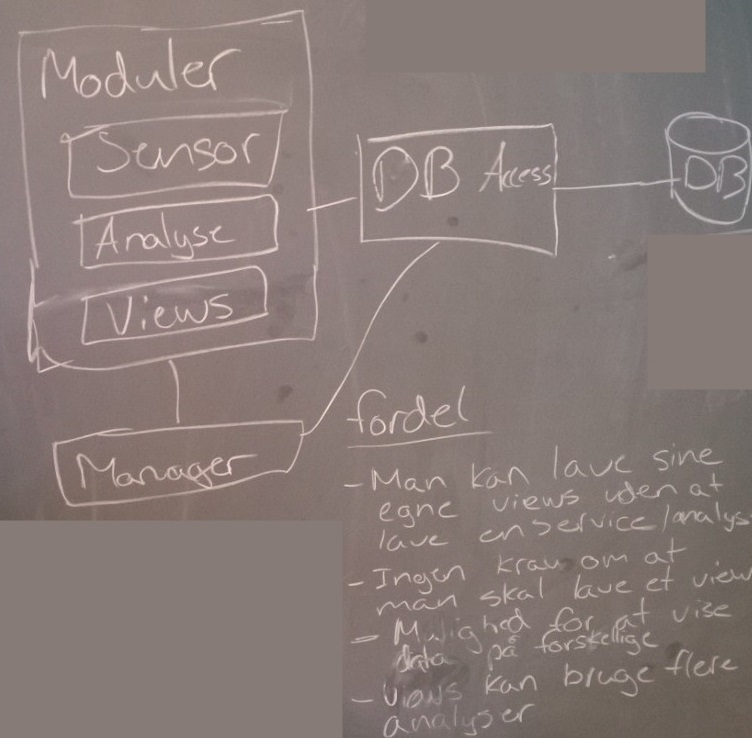
\includegraphics[width=\textwidth]{architecture_draft}
	\caption{Første udkast til arkitektur.}
  \label{arkitektur_udkast_1}
\end{figure}
Som nævnt herover er styrken ved denne arkitektur, den modulære opbygning af sensorer, analyser og visninger.
Disse lag er derfor alle indholdt i den overordnede komponent \textit{moduler}.
Derudover eksisterer et system, bestående af de resterende tre komponenter, der anvender de moduler der er installeret på den enkelte telefon.
Systemet er altså opbygget uden direkte kendskab til de enkelte moduler, hvilket igen tillader udviklingen af moduler sideløbende med det overordnede system.

Herunder gives en kort beskrivelse af hver af de fire komponenter.
Komponenterne beskrives i rækkefølge af deres indbyrdes afhængighed, således at forståelsen af hver komponent kun afhænger af det læste.

\subsection*{DB}
Denne komponent administrerer data for systemets forskellige moduler.
Data opbevares i en række tabeller i et relationelt database system.
Hvert modul har mulighed for at definere egne tabeller, der alle gemmes i \textit{DB} komponenten.

Til dette projekt er valgt en sqlite database da denne er standard i android.

\subsection*{DB Access}
Denne komponent styrer adgangen til \textit{DB} komponenten så det sker på en ensrettet måde.
\textit{DB Access} holder derudover styr på hvilke komponenter og lag der må skrive og læse fra de enkelte tabeller.

\stefan{som det er nu kan alt skrive til og læse fra alt}

Systemet anvender udelukkende en database placeret på selve mobiltelefonen og er dermed begrænset af de muligheder der er for lagring på den enkelte enhed.
I en fremtidig udvidelse af systemet kunne \textit{DB Access} komponenten tilgå et ekstern lager hvor dele af det administrerede data kan gemmes.
Denne abstraktion forventes at kunne påføres \textit{DB Access} uden at kræve ændringer i de resterende komponenter.

Muligheden for en sådan udvidelse af systemet er ikke undersøgt og der kan derfor naturligt være komplikationer herved, ligesom udvidelsen ikke med sikkerhed kan laves uden påvirkning af de resterende komponenter.

\subsection*{Moduler}
Denne komponent består af de tre forskellige modul-lag.
Til hvert enkelt modul hører en modulbeskrivelse (se \cref{modul_definition}) der beskriver modulets afhængigheder af andre moduler samt hvordan det skal administreres i systemet.

Denne administration består til dels i en definitioner af de tabeller modulet har behov for at få oprettet i \textit{DB} komponenten.
Alle moduler kan skrive til de tabeller de selv definerer, samt læse fra alle andre modulers tabeller.
Adgangskontrollen til tabeller håndteres i \textit{DB Access} komponenten som alle moduler anvender til database adgang.

\stefan{skal der være eksempler på sensorer, moduler, etc?}
\mikkel{jeg har tilføjet et eksempel på sammenhængende moduler i den introducerende tekst. skal vi have yderligere?}
\paragraph{Sensor} \textit{Sensor}laget indeholder alle de moduler der logger data fra sensorer eller logger data fra applikationer.

\paragraph{Analyse}
\textit{Analyse}laget indeholder alle moduler der bruger et antal \textit{sensor}moduler og analyserer det data for derefter at gemme det i en databasetabel.

\paragraph{Views}
\textit{Views}laget indeholder alle moduler der gør det muligt at visualisere de analyserede data.
Den angiver hvilke og hvor mange datatyper den kan vise.

\subsection*{Manager}
Denne komponent står for at holde styr på hvilke moduler der er installeret og opretter tabeller i databasen for dem.
\textit{Manageren} indeholder også et GUI så brugeren kan tilføje og fjerne moduler.
\textit{Manageren} har også logikken for hvilke \textit{analyse} moduler der kan vises i hvilke \textit{views}.
Desuden indeholder \textit{manageren} også et JSON skema for hver modul-type i \textit{moduler} komponenten.
\stefan{et eller flere skemaer? Muligvis har views anderledes skema, men analyse og sensorer har det samme}